\chapter{Manual de Usuario}
\label{ch:manual_usuario}

En este apéndice se detalla el manual de usuario correspondiente al sistema desarrollado, guiando paso a paso en el proceso de uso de la plataforma. Se asume que la \ac{FPGA} ya tiene el diseño programado en su memoria de configuración; este manual cubre por tanto la puesta en marcha del hardware y el uso del software de PC.

% -----------------------------------------------------------------
\section{Requisitos del sistema}
\label{sec:requisitos}

Antes de iniciar la instalación, hay que cumplir con los siguientes requisitos previos en su equipo:

\begin{itemize}
    \item \textbf{Sistema operativo:} Windows~11, con un mínimo de 8~GB de RAM.
    \item \textbf{Basys~3:} Basys~3 con el \textit{bitstream} de VICON ya programado en su memoria de configuración, conectada al sensor MT9V111 y al chip FT232H (módulo UM232H-B) utilizando los conectores \textit{Pmod} indicados en la Figura~\ref{fig:arq_fisica}.
    \item \textbf{Driver D2XX:} controlador D2XX de FTDI instalado en el PC (disponible en \url{https://ftdichip.com/drivers/d2xx-drivers/}), necesario para que la aplicación de PC acceda al FT232H.
    \item \textbf{Cable USB:} un cable USB~2.0 que conecte el módulo UM232H-B directamente a un puerto del PC. Se recomienda evitar conectarlo a través de un \textit{hub} USB, ya que puede introducir latencias adicionales en la recepción del vídeo.
\end{itemize}

\textit{Antes de encender o alimentar la placa}, comprobar la posición del \textit{jumper} de modo de arranque (\texttt{JP1}). Para que la Basys~3 cargue el diseño desde su memoria de configuración no volátil, dicho \textit{jumper} debe situarse en la posición \texttt{QSPI}; en la posición \texttt{USB} la placa esperaría en su lugar una programación por JTAG desde Vivado.

% -----------------------------------------------------------------
\section{Instalación y configuración}
\label{sec:instalacion}

Se deben seguir los pasos descritos a continuación para preparar el software de visualización:

\subsection{Descarga del código fuente}
Clonar el repositorio oficial del proyecto desde \url{https://github.com/carlosmgj/VICON}

\subsection{Configuración del módulo FT232H}
El módulo UM232H-B debe tener su \ac{EEPROM} configurada en modo \textbf{FT245 FIFO} para poder operar en modo \textit{Synchronous FIFO}. Esta configuración solo es necesaria una vez por dispositivo:

\begin{enumerate}
    \item Instalar la utilidad \textbf{FT\_Prog} de FTDI (requiere el driver D2XX ya instalado).
    \item Conectar el UM232H-B al PC y, en FT\_Prog, pulsar \textit{Scan and Parse} para detectar el dispositivo.
    \item Navegar hasta \texttt{FT EEPROM~$\rightarrow$~Hardware Specific~$\rightarrow$~Port~A~$\rightarrow$~Hardware} y cambiar el modo de \texttt{UART} a \texttt{245~FIFO}.
    \item Programar la \ac{EEPROM} (icono del rayo) y, al finalizar, desconectar y vuelva a conectar el módulo para que el sistema operativo lo reconozca con la nueva configuración.
\end{enumerate}

\subsection{Compilación de la aplicación de PC}
La aplicación \texttt{vicon\_view} se distribuye como un ejecutable y por tanto no hace falta tener las dependencias instaladas. Únicamente serían necesarias para la compilación de la aplicación.
La ruta del ejecutable es: \url{VICON/07-Versions/3.0/GUI/vicon_gui.exe}
% -----------------------------------------------------------------
\section{Guía de uso de la aplicación}
\label{sec:guia_uso}

\subsection{Inicio de la aplicación}
Con la Basys~3 encendida, el sensor conectado y el módulo FT232H enlazado al PC por USB, ejecutar \texttt{vicon\_view}. La aplicación abre el dispositivo FT232H a través del \textit{driver} D2XX y comienza a recibir el flujo de vídeo sintético de forma automática; no es necesario ningún paso adicional de emparejamiento o configuración del enlace.

\subsection{Descripción de la interfaz}
Una vez iniciada la interfaz de usuario, se presentan dos zonas principales:

\begin{enumerate}
    \item \textbf{Ventana de vídeo:} muestra en tiempo real el fotograma recibido desde la \ac{FPGA} en escala de grises, junto con la tasa de fotogramas por segundo (\ac{FPS}) actual.
    \item \textbf{Panel de control:} Se encuentran los controles para enviar comandos a la \ac{FPGA}, descritos en la Tabla~\ref{tab:comandos_gui}.
\end{enumerate}

Por defecto, la interfaz muestra el video sintético generado para validar la comunicación entre el sensor y el Host a través de la FPGA como se ve en la Figura~\ref{fig:GUI1}:

\begin{figure}[htbp]
    \centering
    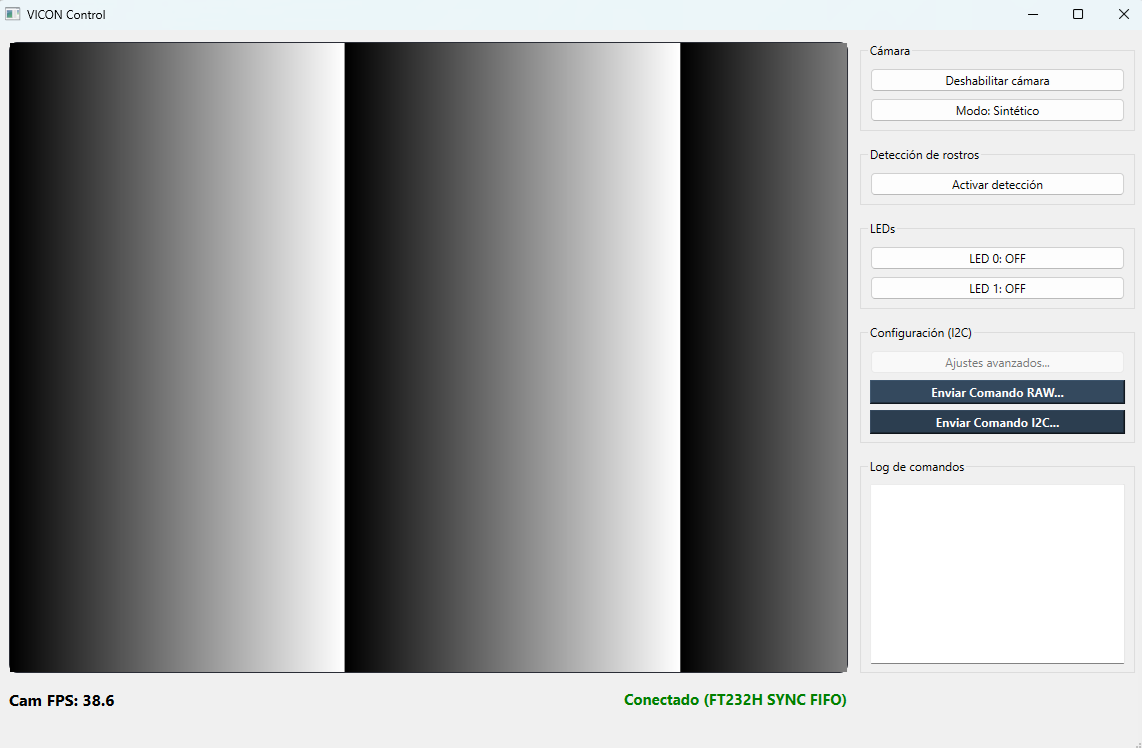
\includegraphics[width=\textwidth]{gfx/vicon_view_gui1.png}
    \caption{Estado Inicial de la Interfaz Gráfica de Usuario.}
    \label{fig:GUI1}
\end{figure}

Para configurar los FPS de la imágen a mínimo 30fps, se deberá configurar el registro I2C correspondiente mandando la trama 1 0x37 0x0080 (Ver Figura~\ref{fig:GUI2}). Este paso se puede realizar antes o después de cambiar el modo de la imágen. 

\begin{figure}[htbp]
    \centering
    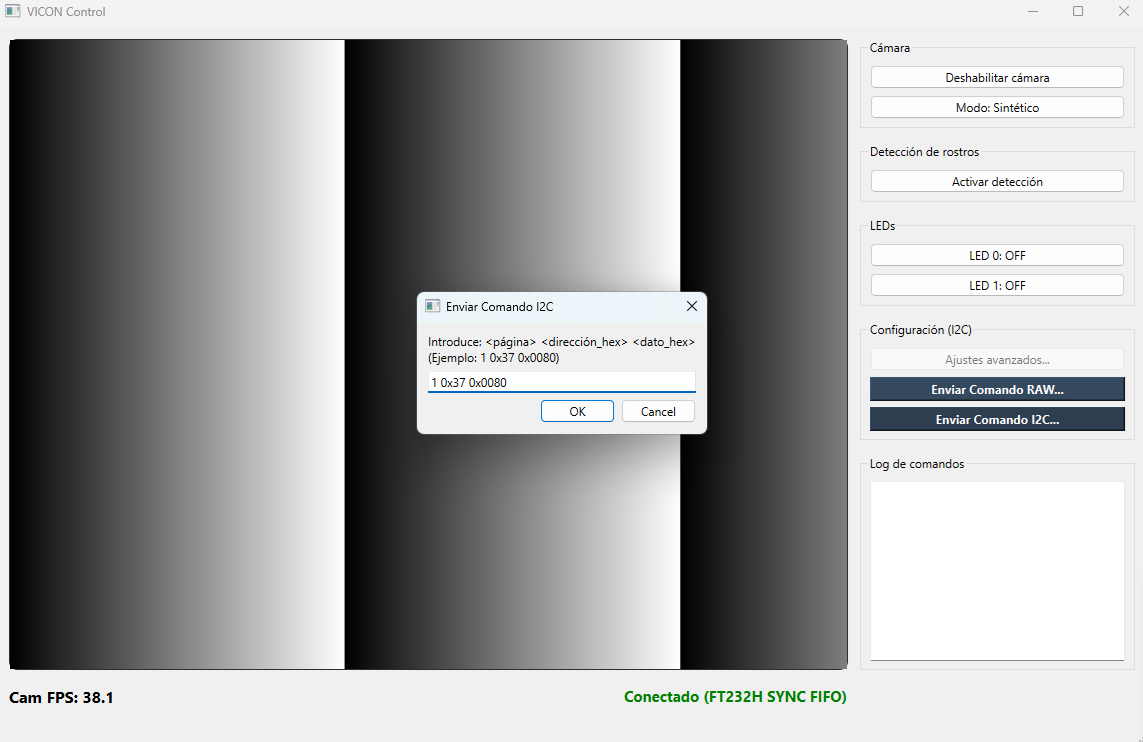
\includegraphics[width=\textwidth]{gfx/vicon_view_gui2.png}
    \caption{GUI: envío de comando I2C para configurar >30fps.}
    \label{fig:GUI2}
\end{figure}

Si a continuación habilitamos la imagen del sensor real y la detección de rostros, el software remarcara la/s cara/s que detecte en la imagen. En la Figura~\ref{fig:GUI3} se puede ver el resultado de presentar al sensor una foto en una tablet con múltiples caras. 

\begin{figure}[htbp]
    \centering
    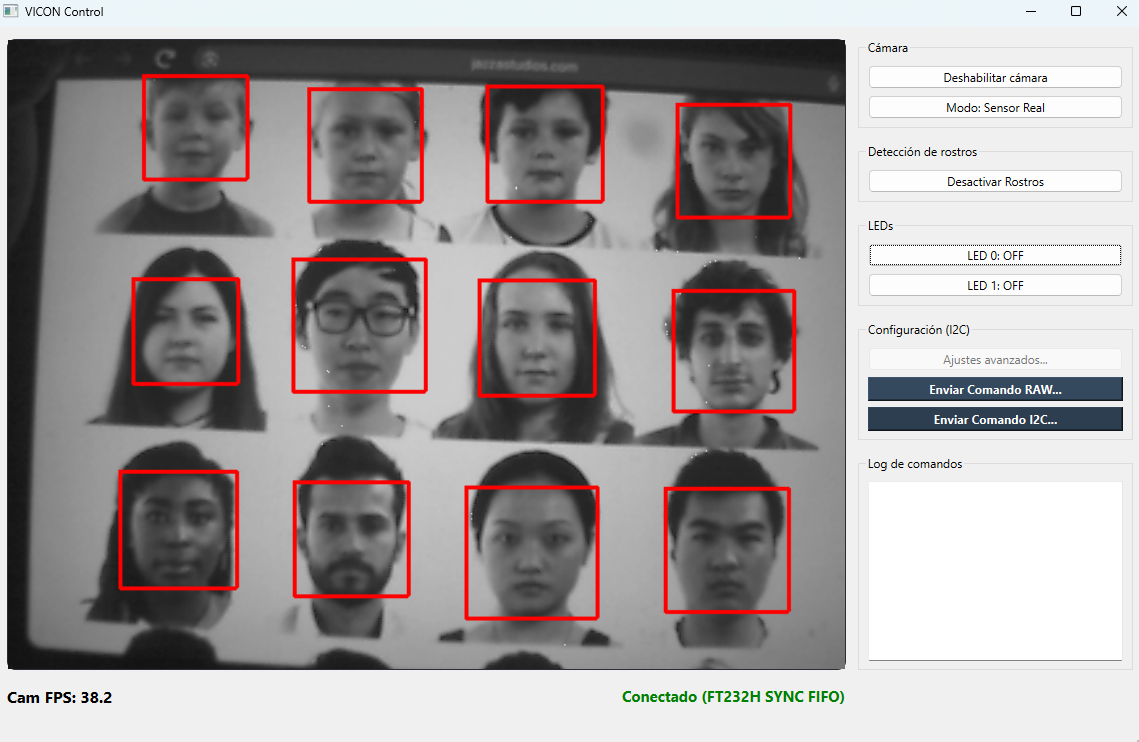
\includegraphics[width=\textwidth]{gfx/vicon_view_gui3.png}
    \caption{GUI: envío de comando I2C para configurar >30fps.}
    \label{fig:GUI3}
\end{figure}

\begin{table}[H]
\centering
\caption{Comandos disponibles desde la interfaz de \texttt{vicon\_view}.}
\label{tab:comandos_gui}
\begin{tabular}{>{\raggedright\arraybackslash}p{3cm}>{\raggedright\arraybackslash}p{9.5cm}}
\rowcolor[HTML]{156082}
{\color{white}\textbf{Comando}} & {\color{white}\textbf{Efecto}} \\
\rowcolor[HTML]{C0E6F5}
LED & Conmuta el estado de un LED de la Basys~3, útil como comprobación rápida de que el canal de comandos PC$\rightarrow$FPGA funciona. \\
Activar/desactivar captura & Detiene o reanuda la transmisión de vídeo desde la \ac{FPGA} sin necesidad de desconectar el enlace USB. \\
\rowcolor[HTML]{C0E6F5}
Imagen sintética & Conmuta entre el sensor MT9V111 y el generador interno de imagen sintética, útil para validar el resto de la cadena sin depender de la cámara física. \\
Escritura de registro I2C & Permite escribir un valor en un registro concreto del sensor (página, dirección y dato), para ajustar su configuración en caliente. \\
\end{tabular}
\end{table}

% -----------------------------------------------------------------
\section{Resolución de problemas (\textit{troubleshooting})}
\label{sec:problemas}

En la Tabla~\ref{tab:errores_frecuentes} se resumen los errores más habituales y las acciones recomendadas para su resolución.

\begin{table}[htbp]
\centering
\caption{Problemas frecuentes y soluciones.}
\label{tab:errores_frecuentes}
\begin{tabular}{|p{3.8cm}|p{4.6cm}|p{4.6cm}|}
\hline
\rowcolor[HTML]{156082}
{\color{white}\textbf{Error}} & {\color{white}\textbf{Causa probable}} & {\color{white}\textbf{Solución recomendada}} \\ \hline
No se ven los LEDs encendidos al arrancar la placa. & \textit{Jumper} de modo mal colocado. & Situar el \textit{jumper} \texttt{JP1} en modo \texttt{QSPI} antes de alimentar la placa. \\ \hline
La aplicación no detecta el FT232H. & Windows ha instalado automáticamente el \textit{driver} VCP (puerto serie virtual) en lugar del D2XX. & Reinstalar el \textit{driver} D2XX desde el Administrador de dispositivos, seleccionando manualmente la carpeta de instalación de FTDI. \\ \hline
FT\_Prog no reconoce el dispositivo al configurar la \ac{EEPROM}. & Conflicto entre el \textit{driver} D2XX y otro \textit{driver} (p.~ej. \texttt{libusb}) instalado previamente sobre el mismo dispositivo. & Reinstalar el \textit{driver} D2XX y volver a conectar el cable antes de reintentar con FT\_Prog. \\ \hline
El vídeo se congela o aparecen fotogramas corruptos de forma intermitente. & Sobreescritura de la \ac{FIFO} interna por una latencia de lectura excesiva en el PC (agravada si el FT232H está conectado a través de un \textit{hub} USB). & Conectar el módulo directamente a un puerto USB del equipo, sin \textit{hubs} intermedios. \\ \hline
\end{tabular}
\end{table}